It's very useful to note that we can expand angular dependence from the Legendre polynomials $P_l$ in terms of spherical harmonics, i.e.
\begin{equation}\label{eqn:legendreandspherical}
    P_l(\uv r \cdot \uv r') = \frac{4\pi}{2l+1} \sum_{m=l}^l Y_{lm}^*(\theta',\phi') Y_{lm}(\theta, \phi).
\end{equation}
That is, we can express an arbitrary angular dependence in terms of spherical harmonics. For instance,
\begin{equation}\label{eqn:angularexpn}
    f(\theta,\phi;\theta',\phi') = \sum_{l'=0}^\infty \sum_{m=-l'}^{l'} A_{l' m}(\theta',\phi') Y_{l',m}(\theta, \phi),
\end{equation}
where we treat the $A_{l'm}$ as coefficients which depend on ``fixing'' some choice of $\theta',\phi'$. That is, $A_{l'm}$ is like picking a choice of coordinates, and in particular choosing $f$ to be the Legendre polynomial $f(\theta,\phi;\theta',\phi')=P_l(\theta,\phi;\theta',\phi')$ tells us that
\begin{equation}
    P_l (\theta, \phi; \theta', \phi') = \sum_{m=l}^l A_{lm}(\theta',\phi') Y_{lm}(\theta, \phi),
\end{equation}
where
\begin{equation}
    A_{lm}(\theta',\phi') = \frac{4\pi}{2l+1} Y_{lm}^*(\theta',\phi').
\end{equation}
That is, the only terms in the sum \eqref{eqn:angularexpn} we need are for $l'=l$.

The spherical harmonics $Y_{lm}$ are polynomials in $x,y,z$ of degree $l$. All terms in a given spherical harmonic either have even degree or odd degree. Moreover, we can make all terms have degree $l$ by inserting $x^2+y^2 +z^2$s, since this is equal to $r^2=1$ on the unit sphere. For instance,
\begin{equation}
    P_2 = \frac{3}{2}z^2 - \frac{1}{2} = \frac{3}{2} z^2 - \frac{1}{2}(x^2+y^2+z^2) = z^2 - \frac{1}{2}x^2 -\frac{1}{2}y^2.
\end{equation}
Hence we can always increase the power of a term by $2$. Similarly $Y_{3m}$ will contain terms like 
\begin{equation*}
    x^3, y^3, z^3, xyx, xxy, yxx, \dots,
\end{equation*}
and this sort of counting argument is exactly analogous to our multipole expansion and how elements of the tensor were related by symmetry. Then the $x^2+y^2+z^2=1$ constraint gives us our trace constraints.

We could also make a transformation $x\to x'\cos\alpha + y' \sin \alpha, y \to -x' \sin\alpha + y'\cos\alpha$, and we see that under such rotations, the orders of the terms in $Y_{lm}$ don't change. It follows that rotations don't mix $Y_{lm}$s between different orders $l$.

Let's now make an argument from completeness using a 2D delta function defined on the surface of a sphere. We'll write it in terms of unit vectors rather than angles to avoid prefactors of the sphere area. Hence we shall assert that the delta function can be expanded in this way,
\begin{equation}
    \delta(\uv v - \uv w)= \sum_{l=0}^\infty \sum_{m=-l}^l c_{lm}(\uv w) Y_{lm}(\uv v)
\end{equation}
where $Y_{lm}(\uv v)$ indicates the spherical harmonic as a function of the angular coordinates of $\uv v$. The (as yet undetermined) coefficients $c_{lm}$ depend on $\uv w$, just as $A_{l'm}$ depended on $\theta',\phi'$.

Now we observe that by the orthonormality of the spherical harmonics,
\begin{equation}
    \int d\Omega_v \sum_{l=0}^\infty \sum_m c_{lm} Y_{lm} (\uv v) Y_{l'm'}^*(\uv v) = c_{lm} \delta_{ll'}\delta_{mm'} = c_{l'm'}(\uv w).
\end{equation}
But this is equivalent to
\begin{equation}
    \int d\Omega_v \paren{\sum_{l=0}^\infty \sum_m c_{lm} Y_{lm} (\uv v)} Y_{l'm'}^*(\uv v)=\int d\Omega_v \delta(\uv v - \uv w) Y_{l'm'}^* Y_{l'm'}^*(\uv v) = Y^*_{l'm'}(\uv w)
\end{equation} 
It follows that
\begin{equation}
    c_{lm}(\uv w) = Y^*_{lm}(\uv w),
\end{equation}
so
\begin{equation}
    \boxed{\delta (\uv v - \uv w) = \sum_{l=0}^\infty \sum_{m=-l}^l Y_{lm}(\uv v) Y_{lm}^*(\uv w).}
\end{equation}
If we choose $\uv w = \uv z$, i.e. we fix $\uv w$ to point along the $z$ axis, then we have \emph{cylindrical} symmetry, not just spherical. But only the $m=0$ spherical harmonics have cylindrical symmetry, so in fact
\begin{equation}
    \delta(\uv v - \uv z) = \sum_{l=0}^\infty Y_{l0} (\uv v) Y_{l0}^*(\uv z).
\end{equation}
Moreover, note that $P_l(\cos\theta =0) =1$,
\begin{equation}
    Y_{l0} = \sqrt{\frac{2l+1}{4\pi}} P_l,
\end{equation}
so it follows that
\begin{equation}
    \delta(\uv v - \uv z) = \sum_{l=0}^\infty \frac{2l+1}{4\pi} P_l(\uv v \cdot \uv z).
\end{equation}
It follows that since the LHS of this expression depends only on the difference $\uv v - \uv z$ and the RHS depends only on the dot product $\uv v \cdot \uv z$, this difference is independent of rotating our choice of coordinates, which means that in fact
\begin{equation}
    \boxed{\delta(\uv v - \uv w) = \sum_{l=0}^\infty \frac{2l+1}{4\pi} P_l(\uv v\cdot \uv w).}
\end{equation}
Equating the boxed equations and taking this order by order in $l$, we find precisely that
\begin{equation}
    P_l (\uv r \cdot \uv r') = \frac{4\pi}{2l+1} \sum_{m=-l}^l Y_{lm}^* (\theta', \phi') Y_{lm}(\theta,\phi),
\end{equation}
which is none other than Eqn.~\eqref{eqn:legendreandspherical}.

Back to the physics. Recall that Coulomb's law gives us scalar potentials as
\begin{equation}
    \varphi(\vec r) = \frac{1}{4\pi \epsilon_0} \int d^3 r' \frac{\rho(\vec r')}{|\vec r - \vec r'|}.
\end{equation}
There's a nice expansion we can use for this inverse separation:
\begin{equation}
    \frac{1}{|\vec r - \vec r'|} = \frac{1}{r} \sum_{l=0}^\infty \paren{\frac{r'}{r}}^l P_l (\uv r \cdot \uv r'),\quad r' < r.
\end{equation}
This is really a very sensible way to \emph{define} the Legendre polynomials. The RHS is an expansion in increasing powers of $1/r$, and purely on dimensional grounds, the RHS must have dimensions of $1/\text{distance}$, which means that increasing powers of $1/r$ must be accompanied by powers of $r'$. That is, we need powers of $r'/r$. Plugging in our expansion \eqref{eqn:legendreandspherical} we have
\begin{equation}
    \frac{1}{|\vec r-\vec r'|} = \frac{1}{r} \sum_{l=0}^\infty \sum_{m=-l}^l \frac{4\pi}{2l+1} \paren{\frac{r'}{r}}^l Y_{lm}(\theta,\phi) Y_{lm}^* (\theta',\phi').
\end{equation}
Last time, we saw that
\begin{equation}
    \varphi(\vec r) = \frac{1}{4\pi \epsilon_0} \sum_{l=0}^\infty \sum_{m=l}^l A_{lm} \frac{Y_{lm}(\theta,\phi)}{r^{l+1}} \implies A_{lm} = \int d^3 r' \frac{4\pi}{2l+1} r'^l Y_{lm}^*(\theta',\phi') \rho(\vec r').
\end{equation}
The interior solution for Laplace's equation (i.e. the one that doesn't diverge as $r\to 0$) just replaces $\frac{r'{}^l}{r^{l+1}} \to \frac{r^l}{(r')^{l+1}},$ and then the $A_{lm}$s are modified.

\subsection*{Conductors}
For our purposes, we will use the terms conductors and metals interchangeably. The charge carriers in a conductor reorganize themselves to respond to external applied fields. Specifically, they configure themselves so that the electric field inside is zero (equivalently, this minimizes the energy in the field). Thus $\vec E = 0$ inside. On the surface, the electric field is perpendicular to the surface. If this weren't the case, the charge would reshuffle to cancel this.%
    \footnote{At least in the absence of an external magnetic field.}
To sum up,
\begin{gather}
    \vec E = 0 \text{ inside},\\
    E_\parallel = 0 \text{ on surface.}
\end{gather}
It follows from Gauss's law and the definition of potential that
\begin{equation}
    \rho=0, \quad \varphi = \text{constant inside}.
\end{equation}
Let's work out the classic example of a neutral conducting sphere in a constant applied field $E_0$. See Fig.~\ref{fig:zangwill_fig_5_2}. The total field in the sphere is therefore the sum of the applied field and the induced field from the rearranged charges in the sphere.

That is, if the applied field is
\begin{equation}
    \vec E_0 = E_0 \uv z,
\end{equation}
then the self-field inside must be $-E_0 \uv z$. The potential from the induced charge is%
    \footnote{This is clearly not constant! Nor should it be. The total potential is constant, and it is the sum of this induced potential and the potential sourcing the applied field.}
\begin{equation}
    \varphi_\text{self} (r<R,\theta) = E_0 z = E_0 r\cos\theta.
\end{equation}
A priori, the self-field outside is then
\begin{equation}
    \varphi_\text{self}(r>R, \theta) = \frac{1}{4\pi \epsilon_0} \bkt{\frac{A_0}{r} + \frac{A_1}{r^2}P_1(\cos\theta) + \frac{A_2}{r^3} P_2(\cos\theta) + \dots}
\end{equation}
We can now use matching conditions. The potential is continuous, so if we take $r=R$ and set $\varphi_\text{self}$ inside equal to $\varphi_\text{self}$ outside, then
\begin{equation}
    E_0 R \cos\theta = \frac{1}{4\pi \epsilon_0} \frac{A_1}{R^2} \cos\theta.
\end{equation}
By the orthogonality of the Legendre polynomials, we can just match order by order in $P_l$, and if we solve for $A_1/4\pi \epsilon_0$, then
\begin{equation}
    \varphi_\text{self}(r\geq R, \theta) = E_0 R^3 \frac{\cos\theta}{r^2}.
\end{equation}
This is \emph{exactly} the field of a dipole.
The quantity $\vec p = 4\pi R^3 \epsilon_0 \vec E$ is the dipole moment of this sphere, where $\alpha = 4\pi R^3$ is called the polarizability. In general, more complicated shapes will have a vanishing monopole moment but some some of higher multipole moments.

\begin{figure}
    \centering
    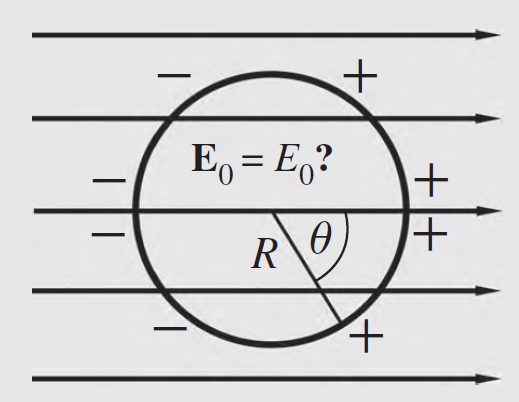
\includegraphics{2020/01/zangwill_fig_5_2.png}
    \caption{Zangwill Fig.~5.2.}
    \label{fig:zangwill_fig_5_2}
\end{figure}

Suppose now we have some strangely-shaped conductor with a cavity machined out of it, and we place a small (say, positive) charge inside the cavity. Well, what happens to the charge in the conductor? Clearly the inside surface of the cavity must rearrange itself to cancel the field within the conductor. That takes some net negative charge on the inside surface. That is, negative charge accumulates to shield the interior. That charge had to come from somewhere, though. There must be a net positive charge on the exterior surface which rearranges itself in some energetically favorable way. The neat thing is that the solution on the exterior surface doesn't depend at all on the shape of the cavity, or where the charge is placed inside. This is what we mean by shielding. Our conductor hides the details of the interior and reveals only the net charge contained within.